%for a more compact document, add the option openany to avoid
%starting all chapters on odd numbered pages
\documentclass[12pt]{cmuthesis}

% This is a template for a CMU thesis.  It is 18 pages without any content :-)
% The source for this is pulled from a variety of sources and people.
% Here's a partial list of people who may or may have not contributed:
%
%        bnoble   = Brian Noble
%        caruana  = Rich Caruana
%        colohan  = Chris Colohan
%        comar    = Cyrus Omar
%        jab      = Justin Boyan
%        josullvn = Joseph O'Sullivan
%        jrs      = Jonathan Shewchuk
%        kosak    = Corey Kosak
%        mjz      = Matt Zekauskas (mattz@cs)
%        pdinda   = Peter Dinda
%        pfr      = Patrick Riley
%        dkoes = David Koes (me)

% My main contribution is putting everything into a single class files and small
% template since I prefer this to some complicated sprawling directory tree with
% makefiles.

% some useful packages
\newcommand{\todo}[1]{\textcolor{red}{TODO: #1}}
\usepackage{times}
\usepackage{fullpage}
\usepackage{graphicx}
\usepackage{amsmath}
\usepackage{amssymb}
\usepackage{multirow}
\usepackage{booktabs}
\usepackage[numbers,sort]{natbib}
\usepackage[backref,pageanchor=true,plainpages=false, pdfpagelabels, bookmarks,bookmarksnumbered,
%pdfborder=0 0 0,  %removes outlines around hyper links in online display
]{hyperref}
\usepackage{subfigure}

% Approximately 1" margins, more space on binding side
%\usepackage[letterpaper,twoside,vscale=.8,hscale=.75,nomarginpar]{geometry}
%for general printing (not binding)
\usepackage[letterpaper,twoside,vscale=.8,hscale=.75,nomarginpar,hmarginratio=1:1]{geometry}

% Provides a draft mark at the top of the document. 
\draftstamp{\today}{DRAFT}

\begin {document} 
\frontmatter

%initialize page style, so contents come out right (see bot) -mjz
\pagestyle{empty}

\title{ %% {\it \huge Thesis Proposal}\\
{\bf Dissecting Reinforcement Learning: Mechanisms Behind Compositional Reasoning in LLMs}}
\author{\bf Gyeongwon James Kim}
\date{May 2026}
\Year{2026}
\trnumber{CMU-CS-26-TBD}

\committee{
Chenyan Xiong, Chair \\
Aditi Raghunathan \\
}

\support{}
\disclaimer{}

% copyright notice generated automatically from Year and author.
% permission added if \permission{} given.

\keywords{Large Language Models, Reasoning Models, Reinforcement Learning, Compositional Generalization}

\maketitle

\begin{dedication}
For my family and friends who supported me through this journey.
\end{dedication}

\pagestyle{plain} % for toc, was empty

%% Obviously, it's probably a good idea to break the various sections of your thesis
%% into different files and input them into this file...

\begin{abstract}
% Hook 
% Motivation
Recently, Large Reasoning Models (LRMs) have achieved impressive performance on a variety of reasoning tasks, including mathematics and code generation. Their long chains of reasoning enable scaling of inference-time computation, allowing them to solve increasingly complex problems. LRMs are typically post-trained from base models using supervised fine-tuning (SFT), reinforcement learning (RL), or a combination of both. RL is often hypothesized to be a key driver of reasoning ability, as it enables models to explore and discover new solutions. However, recent work suggests that RL may instead concentrate probability mass on existing solutions.
% Problem
The mechanisms by which RL leads to reasoning ability remain poorly understood. In this thesis, we study RL training mechanisms through the lens of compositional generalization—a key sub-skill of reasoning that involves combining atomic skills to solve more complex problems.
% Findings
We find that RL-trained models substantially outperform those trained with standard SFT on this task. To isolate the effects of RL, we decompose it into three components: on-policy data, the use of negative samples, and objective design. By ablating each component, we establish a progression from SFT to RL and identify their respective contributions. Empirically, we find that both on-policy data and negative samples are critical for the emergence of compositional generalization, while objective design choices (e.g., group normalization) have a relatively small impact.
% conclusion
Our findings suggest that effective post-training of LLMs requires understanding and carefully designing the individual components of the training pipeline, rather than treating RL as a monolithic improvement.
\end{abstract}

\begin{acknowledgments}

\end{acknowledgments}



\tableofcontents
\listoffigures
\listoftables

\mainmatter

%% Double space document for easy review:
%\renewcommand{\baselinestretch}{1.66}\normalsize

% The other requirements Catherine has:
%
%  - avoid large margins.  She wants the thesis to use fewer pages, 
%    especially if it requires colour printing.
%
%  - The thesis should be formatted for double-sided printing.  This
%    means that all chapters, acknowledgements, table of contents, etc.
%    should start on odd numbered (right facing) pages.
%
%  - You need to use the department standard tech report title page.  I
%    have tried to ensure that the title page here conforms to this
%    standard.
%
%  - Use a nice serif font, such as Times Roman.  Sans serif looks bad.
%
% Other than that, just make it look good...


\chapter{Introduction}
% Hook
Recent advances in large language model post-training have produced a new class of systems capable of solving problems that once seemed far beyond reach: competition mathematics, graduate-level science questions, and complex multi-step code generation.
The defining ingredient is reinforcement learning with verifiable rewards (RLVR), exemplified by DeepSeek-R1 \citep{deepseek-aiDeepSeekR1IncentivizingReasoning2025} and a wave of follow-up work.
In these systems, a language model generates candidate solutions, a lightweight verifier checks correctness, and the model is updated to produce better solutions over time without human labels.
As a result, these models can produce multi-chain reasoning traces that allow them to solve increasingly complex problems.

% Need and Gap
Yet the mechanisms behind how RL leads to reasoning ability remain poorly understood.
At least three explanations compete in the literature.
The \emph{sharpening} view holds that RLVR mostly concentrates probability mass on outputs already existing in the base model, improving single-sample accuracy without fundamentally expanding the model's capabilities \citep{yueDoesReinforcementLearning2025}.
The \emph{on-policy} view argues that the key is the alignment between training data and the model's current distribution: because RL continuously generates rollouts from the evolving policy, it avoids the off-policy bias of static supervised datasets \citep{chenRetainingDoingRole2025,mingOneTokenRolloutGuiding2026}.
The \emph{negative feedback} view emphasizes that unlike SFT, which only reinforces correct demonstrations, RL explicitly penalizes incorrect outputs, driving the model to avoid failure modes \citep{tian_learning_2026}. Other works also find that negative gradients are responsible for the increase in reasoning length, which is necessary for harder problems \citep{setlurE3LearningExplore2025}.
In practice, modern RL pipelines bundle all of these effects together with additional ingredients (KL regularization, variance normalization, entropy shaping, curriculum schedules), making it difficult to attribute gains to any single cause.

% Task
This thesis investigates these mechanisms through the lens of \emph{compositional generalization}: the ability to chain multiple known atomic skills togehter to solve more complex problems.
Compositional generalization is a key ingredient in general reasoning ability. A model solving a complex problem may need to decompose the task into multiple sub-tasks and solve each sub-task sequentially. 
Crucially, the gap between SFT and RL is especially pronounced here: SFT-trained models plateau sharply as composition depth increases, while RL-trained models continue to improve, creating a clean and measurable performance separation \citep{yuanLLMsLearnNewSkills2025, cheng_atomic_2025}.
We use the string-function composition task introduced by \citet{yuanLLMsLearnNewSkills2025}, where the model must predict the output of composed string transformations of increasing depth.

% Method
Our approach decomposes training into two orthogonal axes and varies each independently.
The first axis is \textbf{data}: we compare teacher-generated off-policy data, base-model bootstrapped data, and fully on-policy rollouts, asking how the source of training trajectories affects compositional performance.
The second axis is the \textbf{loss function}: starting from plain SFT (positive samples only), we progressively introduce negative gradient updates, a group mean baseline, and variance normalization, arriving at the full GRPO objective.
By crossing these two axes we construct a grid of training methods that interpolates between standard off-policy SFT and standard GRPO, isolating the contribution of each component and creating a \emph{unified framework} to understand existing post-training paradigms.

% Results
\todo{Add experimental results}


This thesis makes the following contributions:
\todo{Fill in once we have a more complete experimental results}
\begin{enumerate}
    \item \textbf{A unified decomposition framework.} We organize SFT and RL variants under a common framework parameterized by data policy (off-policy to on-policy) and loss function (positive-only to positive+negative to GRPO). This framework clarifies the design space and enables controlled ablations.
    \item \textbf{Demonstration of a large SFT--GRPO gap on compositional generalization.} 
    \item \textbf{On-policy data is a key component}: \todo{}
    \item \textbf{Use of negative gradients is a key component}: \todo{}
\end{enumerate}


\chapter{Related Work}
\section{Training Large Reasoning Models}

The development of reasoning-capable LLMs has been shaped by a progression of post-training techniques.
Early work introduced bootstrapping via self-generated reasoning traces \citep{zelikmanSTaRBootstrappingReasoning2022}, and reinforcement learning from human feedback established RL as a practical post-training tool \citep{ouyangTrainingLanguageModels2022}.
More recently, DeepSeek-R1 \citep{deepseek-aiDeepSeekR1IncentivizingReasoning2025} demonstrated that RL training directly from a base model (zero-RL) can produce strong reasoning behavior, while also finding that a supervised cold-start further stabilizes training and improves downstream performance.
Follow-up systems such as DAPO \citep{yuDAPOOpenSourceLLM2025} introduced objective modifications---clip-higher, entropy-aware rewards, and token-mean normalization---to prevent collapse during prolonged RL training.
SimpleRL-Zoo \citep{zengSimpleRLZooInvestigatingTaming2025} investigated how problem difficulty, output length, and data diversity interact during zero-RL, finding that problem difficulty is critical and that long CoT SFT can suppress exploration.
ProRL \citep{liuProRLProlongedReinforcement2025} studies the regime of extended RL training across many task categories and shows that maintaining exploration throughout requires explicit diversity incentives.

The training dynamics of RL post-training are increasingly well characterized.
Scaling laws for RL post-training follow power-law relationships with compute and data \citep{tanScalingBehaviorsLLM2025}.
Work using synthetic reasoning tasks identifies an ``edge of competence'' effect: RL works best when the base model already has partial competence on a task, and the interplay between pretraining coverage, mid-training distribution, and RL optimization target is a key determinant of compositional generalization \citep{zhangInterplayPreTrainingMidTraining2025}.
A separate line of work identifies specific behavioral primitives---verification, subgoal decomposition, backtracking, backward chaining---that make a model more compatible with RL training \citep{gandhiCognitiveBehaviorsThat2025}.

Despite this progress, most production reasoning systems bundle curriculum schedules, data mixing, reward shaping, and objective modifications into a single pipeline, making it difficult to attribute improvements to specific mechanisms.
This motivates the controlled decomposition approach taken in this thesis.

\section{SFT versus Reinforcement Learning}

Several studies argue that SFT and RL produce qualitatively different distributional changes.
Under a controlled arithmetic task, \citet{chuSFTMemorizesRL2025} find that SFT improves in-distribution accuracy via memorization while RL generalizes to out-of-distribution settings by exploiting underlying model capabilities, and that SFT can stabilize format for downstream RL.
A complementary trajectory-level analysis shows that RL reduces the proportion of incorrect completions while SFT increases the proportion of correct ones: RL compresses wrong trajectories, SFT expands right ones \citep{matsutaniRLSqueezesSFT2025}.
These findings suggest the two methods differ not just in their objective but in which region of the output distribution they reshape.

A second perspective emphasizes the formal relationship between SFT and RL.
SFT on curated data can be viewed as maximizing a lower bound on a sparse-reward RL objective, and importance-weighted SFT tightens this bound and behaves more like RL \citep{qinSupervisedFineTuning2025}.
A unified policy-gradient framework shows that SFT, DPO-style objectives, and RL share a common structure, with key distinctions being the data generating policy, the weighting over outcomes, and the stabilization constraint \citep{lvUnifiedViewLarge2026}.
Combining SFT-style and RL-style signals in a single training stage can be mutually beneficial, with entropy serving as an informative diagnostic of training dynamics \citep{fuSRFTSingleStageMethod2025}.

RL post-training also mitigates catastrophic forgetting.
\citet{chenRetainingDoingRole2025} show that RL forgets prior capabilities significantly less than SFT at matched task performance, attributing this advantage primarily to on-policy data collection rather than to KL regularization or advantage weighting.
\citet{laiReinforcementFineTuningNaturally2026} corroborate this in a continual post-training setting.
More broadly, \citet{wuGeneralizationSFTReinforcement2025} characterize SFT as inducing a directional drift away from prior capabilities that RL counteracts, rather than discovering genuinely new solutions.

While prior works have focused on studying the effects of SFT and RL separately, this thesis takes a more fine-grained approach by analyzing the component-wise contributions of SFT and RL.


\section{Exploration and Sharpening}

An influential debate concerns whether RL primarily \emph{sharpens} existing behaviors or whether it genuinely \emph{explores} new ones.
The sharpening view holds that RL shifts probability mass toward high-reward completions that are already latent in the base model, improving pass@1 while potentially reducing pass@$k$ diversity. Evidence for this view comes from pass@$k$ analyses showing that base models eventually surpass RL-trained models at large $k$ \citep{yueDoesReinforcementLearning2025}, from theoretical characterizations of RLVR as support-constrained optimization that progressively narrows the exploration frontier \citep{wuInvisibleLeashWhy2026}, and from observations of entropy collapse during long training runs \citep{zhaoEchoChamberRL2025}.

The exploration view holds that RL can discover qualitatively new strategies not well represented in the base model.
SimpleRL-Zoo \citep{zengSimpleRLZooInvestigatingTaming2025} argues that exploration exceeds sharpening in accounting for RL gains.
Methods that preserve exploration throughout training include entropy regularization \citep{cuiEntropyMechanismReinforcement2025}, representation-space novelty bonuses \citep{tuylsRepresentationBasedExplorationLanguage2025}, and experience replay strategies that revisit valuable earlier trajectories to prevent mode collapse \citep{douImprovingRLExploration2025,zhangRLEPReinforcementLearning2025,zhanExGRPOLearningReason2025}.


\section{Extrapolation, Chaining, and Compositional Generalization}

Compositional generalization, the ability to recombine known operations in novel arrangements, is a stringent test of systematic reasoning.
LLMs often exhibit compositional deficiencies. Despite strong performance on individual skills, models often fail when those skills must be chained \citep{pressMeasuringNarrowingCompositionality2023,zhaoExploringCompositionalDeficiency2024}.
The OMEGA benchmark operationalizes this by evaluating models that master atomic skills on compositional and transformative combinations, finding substantial failure rates for state-of-the-art models \citep{sunOMEGACanLLMs2025}.
Theoretical analysis shows that data coverage required for multi-hop compositional generalization can grow super-linearly with task diversity, while models that leverage compositional structure or function reuse can generalize more efficiently \citep{abedsoltanTaskGeneralizationAutoRegressive2025}.



The evidence that RL helps with compositional generalization is growing.
Using a synthetic string-function task related to ours, \citet{yuanLLMsLearnNewSkills2025} show that RL enables models to compose $f(g(x))$ from separately learned $f$ and $g$, while off-policy SFT on the composed task fails to generalize.
\citet{motwaniH1BootstrappingLLMs2025} demonstrate that RL with a curriculum of increasing compositional depth improves substantially even at high pass@$k$, suggesting genuine capability acquisition rather than pure sharpening.
Composable chain-of-thought data is critical for enabling models to chain operations systematically, complementing RL supervision \citep{yinLearningComposableChainsofThought2025}.
Work on pre/mid/post-training interactions using a synthetic task identifies an edge of competence in the base model as a prerequisite for RL-driven compositional generalization, and shows that mid-training can bridge the pretraining and post-training distributions to improve this precondition \citep{zhangInterplayPreTrainingMidTraining2025}.


\section{On-Policy Training}

A recurring theme in the SFT-versus-RL literature is the role of on-policy data.
\citet{mingOneTokenRolloutGuiding2026} show that the performance gap between SFT and RL is largely attributable to the off-policy versus on-policy distinction rather than the form of the loss: converting static SFT data into token-level on-policy training consistently outperforms standard SFT.
Taken to its logical conclusion, removing the KL regularization and group-wise normalization from a GRPO objective reduces the algorithm to on-policy SFT while still achieving competitive performance and substantially shorter reasoning traces \citep{zhaoOnPolicySupervisedFineTuning2026}.
Anchored SFT \citep{zhuAnchoredSupervisedFineTuning2026} adds lightweight KL regularization to on-policy training to prevent distributional drift while preserving the tightness of the RL lower bound.

These findings motivate the on-policy axis of our decomposition, but they also leave open a residual question: on-policy SFT does not generally close the full gap to RL, suggesting that other components---negative gradients and objective normalization---provide additional independent signal.
This thesis directly tests whether on-policy data alone is sufficient or whether the combination of on-policy rollouts and negative updates is essential for compositional generalization.

\section{Role of Negative Gradients in Training}

Standard SFT provides only positive gradients: it increases the likelihood of correct trajectories without penalizing incorrect ones.
RL objectives that use advantage weighting implicitly apply negative updates by suppressing below-average completions, but the causal contribution of this negative signal---relative to on-policy data collection---has received limited direct study.

A first challenge is that naive use of negative samples can produce failure modes.
In DPO, the standard contrastive loss can \emph{reduce} the absolute likelihood of preferred responses as long as the relative gap between preferred and dispreferred completions increases \citep{pal_smaug_2024}.
DPO-Positive (DPOP) addresses this by adding a constraint that enforces preferred-response likelihood to remain above the reference model, and consistently outperforms standard DPO across datasets and tasks.
An analogous issue arises in GRPO: \citet{deng_effect_2025} identify \emph{Lazy Likelihood Displacement} (LLD), where the likelihood of correct responses marginally increases or even decreases during training because all tokens in incorrect responses are penalized with equal strength regardless of their contribution.
Their proposed fix, NTHR, down-weights penalties on tokens that cause LLD by using co-occurring correct responses as anchors.
Crucially, they find that negative gradients are not inherently harmful---targeted token-level negative feedback does help---and that the failure mode stems from undifferentiated uniform penalization rather than the negative signal itself.

A second line of evidence shows that negative samples carry genuine learning signal for generalization.
\citet{tian_learning_2026} show that incorporating negative trajectories into SFT---specifically those with valid intermediate reasoning steps but incorrect final answers---yields substantial out-of-domain generalization gains over positive-only training.
Mechanistically, these trajectories boost policy entropy by 35.67\% at inference time, facilitating exploration, and moderate loss descent during training to mitigate overfitting.
The quality of the negative samples further modulates the benefit: \citet{di_not_2026} find that high-quality negatives exhibiting expected format and structural coherence consistently outperform randomly chosen or naively filtered incorrect responses across preference optimization methods.

Taken together, these results establish that the negative gradient is a meaningful and distinct training signal whose effective exploitation requires attention to which tokens are penalized and what quality of negatives are used.
In this thesis, we provide complementary evidence by directly measuring the causal contribution of the negative gradient component in GRPO on compositional generalization, isolating it from the on-policy data effect.


\chapter{Compositional Generalization}
\section{Task Definition}
Compositional generalization is the ability to compose multiple atomic skills to solve a harder problem. Hence, benchmarks for compositional ability define the notion of an atomic skill and construct more complex tasks by composing these skills. Generally, we can measure the difficulty of the task by the amount of composition required to solve it. To make this more concrete, we study a toy task where the goal is to predict the output of functions that map strings to strings \citep{yuanLLMsLearnNewSkills2025}.

\section{Toy Task: String Functions}
\label{sec:string-function}
We study compositional generalization using the string-function setting as proposed in \citet{yuanLLMsLearnNewSkills2025}. The model receives definitions of simple atomic functions and must predict outputs of composed programs.
Note that difficulty is controlled by composition depth. A level-$i$ task requires composing $i$ operations. Figure \ref{fig:string-function} shows an example of string functions in this dataset. The dataset contains 25 unique string functions, split into 13 in the train set and 12 in the eval set. Note that with $i$ composed functions, any combination of string functions is a valid task, leading to exponentially many tasks as a function of $i$.

\begin{figure}[h!]
\centering
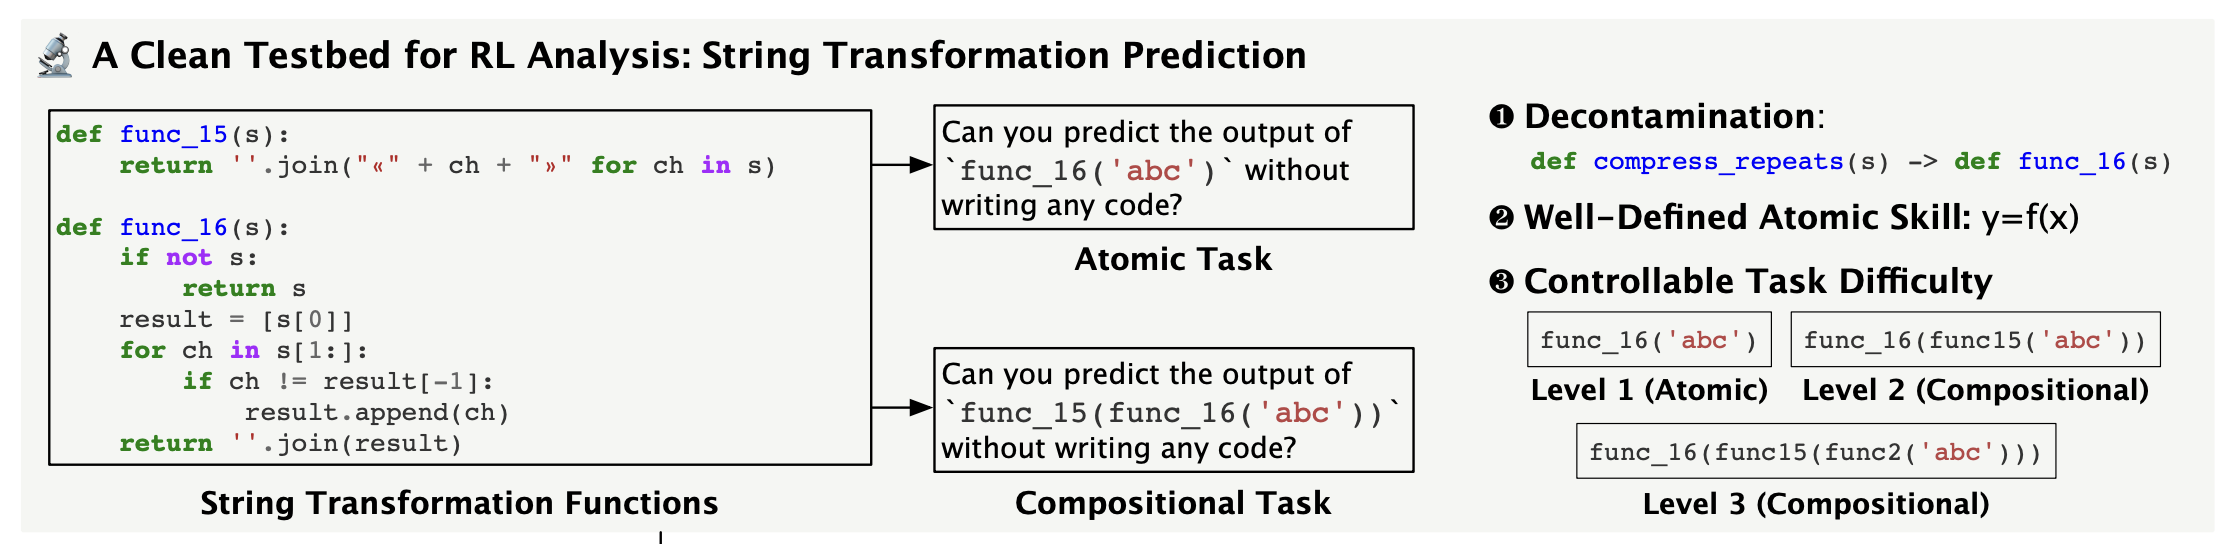
\includegraphics[width=0.9\textwidth]{imgs/string-function.png}
\caption{Figure of String Function Task from original paper \citep{yuanLLMsLearnNewSkills2025}}
\label{fig:string-function} 
\end{figure}


We follow the training protocol proposed in \citet{yuanLLMsLearnNewSkills2025}:
\begin{itemize}
\item \textbf{Stage 1 Training:} In this stage, we train the model on level-1 tasks to ensure that the model has mastered the atomic skills. We call the resulting checkpoint \textbf{Base}, which is used as the starting point for all subsequent training.
\item \textbf{Stage 2 Training:} We train on level-2 tasks using different post-training methods. We use level-2 tasks since they are the lowest difficulty tasks that requires composition.
\item \textbf{Evaluation:} we measure performance on a separate evaluation set on tasks from level 1 to level 8. This allows us to see how performance extrapolates to higher composition levels.
\end{itemize}


\chapter{Decomposing Training Mechanisms}
Our goal is to decompose the training mechanisms across various SFT and RL methods and organize them into a unified framework. As a starting point, we split training into two major components: data and loss function. Data refers to the way we source and select data that will be used for training. Loss function refers to the way we update the model parameters based on the data.

\section{Data}
A key ingredient in post-training is the data. We first consider the source of the data, then consider how we can curate and filter it.

\subsection{Data Source}
One common distinction between methods in RL is whether the data is on-policy or off-policy. On-policy data is generated by the current model, while off-policy data is generated by older models, humans, or teacher models. To study the role of data source, we formalize the following settings:

\begin{itemize}
    \item \textbf{Teacher}: teacher-generated trajectories
    \item \textbf{Bootstrap}: bootstrapped trajectories from the initial model checkpoint
    \item \textbf{Iterative}: bootstrapped trajectories from the previous model checkpoint. We can control the number of model checkpoints, $k$, to use for bootstrapping. If $k=1$, it is the same as Bootstrap-SFT. If $k=\text{number of training steps}$, it is the same as On-policy SFT.
    \item \textbf{On-policy}: on-policy trajectories throughout training
\end{itemize}

In accordance with the literature, we consider the \textbf{Teacher}, \textbf{Bootstrap}, and \textbf{Iterative} settings as Off-policy methods since they make gradient updates based on data from older models or teacher models. However, we can still smoothly transition from Off-policy to On-policy methods by increasing the number of model checkpoints used in the \textbf{Iterative} setting.


\subsection{Data Policy}
Data policy refers to the way we curate data for training. In addition to controlling the data source via on-policy vs off-policy methods mentioned previously, we can also apply additional filtering strategies to the data. For verifiable tasks, it is common practice to filter based on correctness ratios or trajectory lengths.
For example, when training with GRPO, we can filter out groups that have 100\% accuracy or 0\% accuracy since this will result in a zero update signal.
A common approach in fine-tuning is to use Rejection Fine-Tuning (RFT), which only trains on correct samples.


\section{Decomposing the Loss Function}

We start with the loss function for GRPO. For simplicity, we remove the KL-divergence term.

$$ \ell_{\text{GRPO}}(\theta) = - \mathbb{E}_{(x, \{ y\}^G)} \left[ \frac{1}{G} \Sigma_{i = 1}^G \widehat{A}_i \log \pi_\theta(y_i \vert x) \right]$$

The advantage is defined as: $\widehat{A}_i = \frac{r_i - \mu}{\sigma}$ where $r_i$ is the reward, $\mu$ is the mean reward, and $\sigma$ is the standard deviation of the rewards within the group. Note that our task has a binary reward, so we have $r_i \in \{1, 0\}$.

Consider the loss function for standard supervised fine-tuning on positive samples:

$$ \ell_{\text{SFT}}(\theta) = - \mathbb{E}_{(x, y)} \left[ \frac{1}{T} \sum_{t = 1}^T \log \pi_\theta(y_t \vert x, y_{< t}) \right]$$

For consistency with GRPO, we consider training on multiple rollouts of the same problem instance, which forms a group. Furthermore, we can rewrite the following term:
\[
    \log \pi_\theta(y \vert x) = \Sigma_{t = 1}^T \log \pi_\theta(y_t \vert x, y_{< t})
\]

Then, the loss simplifies to 
\[
    \ell_{\text{SFT}}(\theta) = - \mathbb{E}_{(x, \{y\}^G)} \left[ \frac{1}{G} \sum_{i = 1}^G \frac{1}{T} \log \pi_\theta(y_i \vert x) \right]
\]

Since SFT only uses positive samples, we can think of the loss as:
\[
    \ell_{\text{SFT}}(\theta) = - \mathbb{E}_{(x, \{y\}^G)} \left[ \frac{1}{G} \sum_{i = 1}^G \boldsymbol{1}[r_i = 1] \cdot \frac{1}{T} \log \pi_\theta(y_i \vert x) \right]
\]

To incorporate negative samples, we have the following loss:
\[
    \ell_{\text{POS+NEG}}(\theta) = - \mathbb{E}_{(x, \{y\}^G)} \left[ \frac{1}{G} \sum_{i = 1}^G \boldsymbol{1}[r_i = 1] \cdot \log \pi_\theta(y_i \vert x) - \boldsymbol{1}[r_i = 0] \cdot \log \pi_\theta(y_i \vert x) \right]
\]
This is essentially equivalent to the REINFORCE loss with rewards $r_i \in \{1, -1\}$. Then, we can further add a baseline to the REINFORCE loss where $\mu$ is the mean reward of the group:
\[
    \ell_{\text{REINFORCE+}}(\theta) = - \mathbb{E}_{(x, \{y\}^G)} \left[ \frac{1}{G} \sum_{i = 1}^G (r_i - \mu) \cdot \log \pi_\theta(y_i \vert x) \right]
\]

Finally, we add normalization to get GRPO loss:
\[
    \ell_{\text{GRPO}}(\theta) = - \mathbb{E}_{(x, \{y\}^G)} \left[ \frac{1}{G} \sum_{i = 1}^G \left( \frac{r_i - \mu}{\sigma} \right) \cdot \log \pi_\theta(y_i \vert x) \right]
\]

Another setting used to isolate the effect of negative gradients is to apply a mask to the negative gradients in GRPO \citep{setlurE3LearningExplore2025}.
\[
    \ell_{\text{GRPOMask}}(\theta) = - \mathbb{E}_{(x, \{y\}^G)} \left[ \frac{1}{G} \sum_{i = 1}^G \boldsymbol{1}[r_i = 1] \cdot \left( \frac{r_i - \mu}{\sigma} \right) \cdot \log \pi_\theta(y_i \vert x) \right]
\]

As a unified framework, we can view these loss functions as applying different weights to positive and negative samples. Table \ref{tab:loss_function_comparison} summarizes how different loss functions weight positive and negative samples. 

\begin{table}[h!]
\centering
\begin{tabular}{clcc}
\toprule
\textbf{Use of Negative Samples} & \textbf{Loss Function} & \textbf{Positive Weight} & \textbf{Negative Weight} \\
\midrule
\multirow{2}{*}{No} & SFT & $1$ & $0$ \\
& GRPOMask & $(1 - \mu)/\sigma$ & $0$ \\
\midrule 
\multirow{3}{*}{Yes} & POS+NEG & $1$ & $-1$ \\
& REINFORCE+ & $1 - \mu$ & $- \mu$ \\
& GRPO & $(1 - \mu)/\sigma$ & $-\mu/\sigma$ \\
\bottomrule
\end{tabular}
\label{tab:loss_function_comparison}
\caption{Comparison of loss functions by weights used for positive and negative samples.}
\end{table}

\subsection{DPO}
DPO is another method that uses negative samples. It is defined as:

$$ \ell_{\text{DPO}}(\theta) = - \mathbb{E}_{(x, y^+, y^-)} \left[ \log \sigma\left( \beta \left( \log \frac{\pi_\theta(y^+ \mid x)}{\pi_{\text{ref}}(y^+ \mid x)} - \log \frac{\pi_\theta(y^- \mid x)}{\pi_{\text{ref}}(y^- \mid x)} \right) \right) \right]$$
Intuitively, DPO incentivizes the likelihood of the positive sample to be greater than the likelihood of the negative sample. This does not fit well into our framework since it applies a non-linear function to the difference of the log probabilities.

\chapter{Experiments}
\section{Setup}
We use Llama-3.1-8B-Instruct as the backbone model. As noted in section \ref{sec:string-function}, we train this model on level-1 tasks (Stage 1 Training) to ensure that the model has acquired the atomic skills. We call this checkpoint \textbf{Base}. Stage 1 Training uses Rejection Fine-Tuning (RFT) on 117k samples.
In Stage 2 Training, we train the \textbf{Base} model with various training methods as described in the previous chapter. By evaluating the performance of the model on level-$i$ tasks with $i \ge 2$, we can measure the compositional generalization ability of the model.

\subsection{Matching Compute}
To conduct a fair comparision between methods, we utilize a matched compute setting, where compute is measured by the number of samples used in the training process. For On-policy methods, let $b$ be the batch size and $T$ be the total training steps. For each problem instance, we rollout $G$ samples (this is also the group size in GRPO). Then, the total number of samples used is $bTG$. For Off-policy methods, we use the teacher model or checkpoint model to generate $G$ solutions for $bT$ problem instances, matching the total sample count.

One thing to note is that when we use SFT loss, we only use positive samples. However, we still measure the compute by the total number of samples \emph{before} filtering out the negatives.

By default, we use a batch size of $b=16$ and $T=1200$ training steps, resulting in $19200$ unique problem instances. We use group size of $G=16$, resulting in total sample count of $307200$.


\section{Baselines}
In order to understand the effect of different components, we establish lower and upper bounds for performance. Namely, the standard off-policy SFT method establishes the baseline lower bound performance. On the other hand, standard on-policy GRPO establishes our gold-standard upper bound in performance. Figure \ref{fig:baselines} shows the performance gap, which we hope to close by ablating various components.

\begin{figure}[h!]
\centering
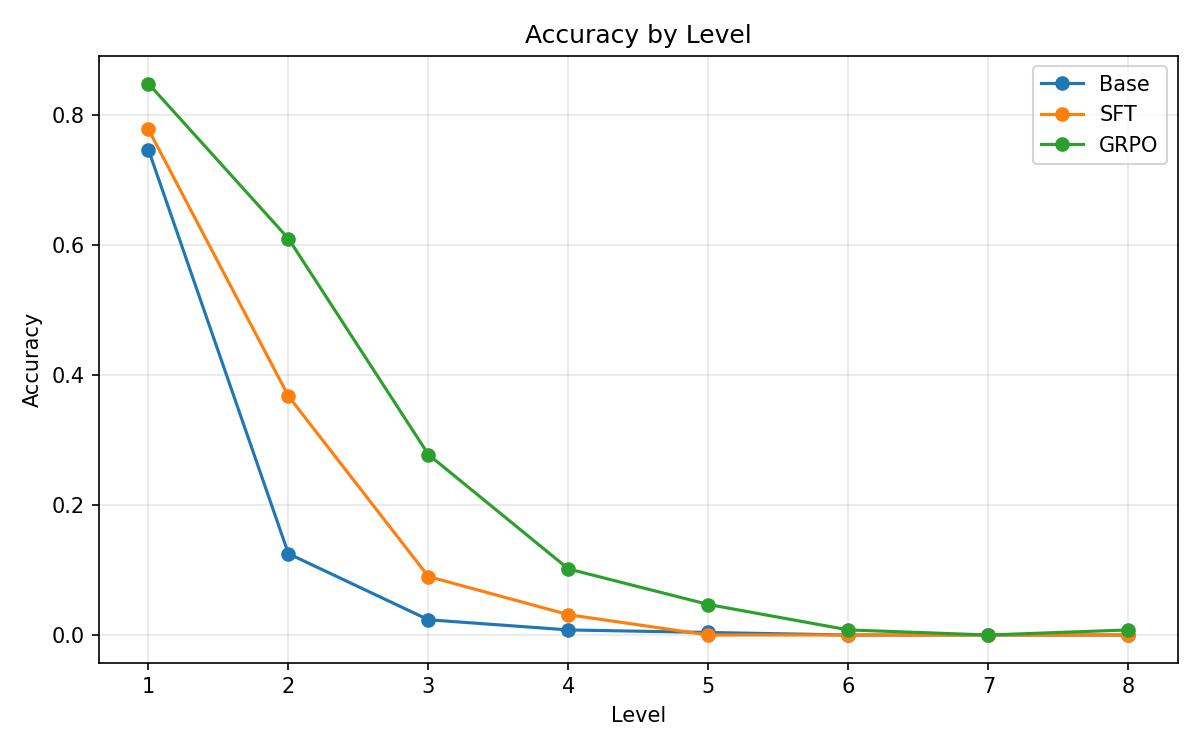
\includegraphics[width=0.8\textwidth]{imgs/baseline.png}
\caption{Accuracy comparing the Base model to 2 training methods: SFT and GRPO}
\label{fig:baselines}
\end{figure}



\section{Data}
\begin{figure}[h!]
\centering
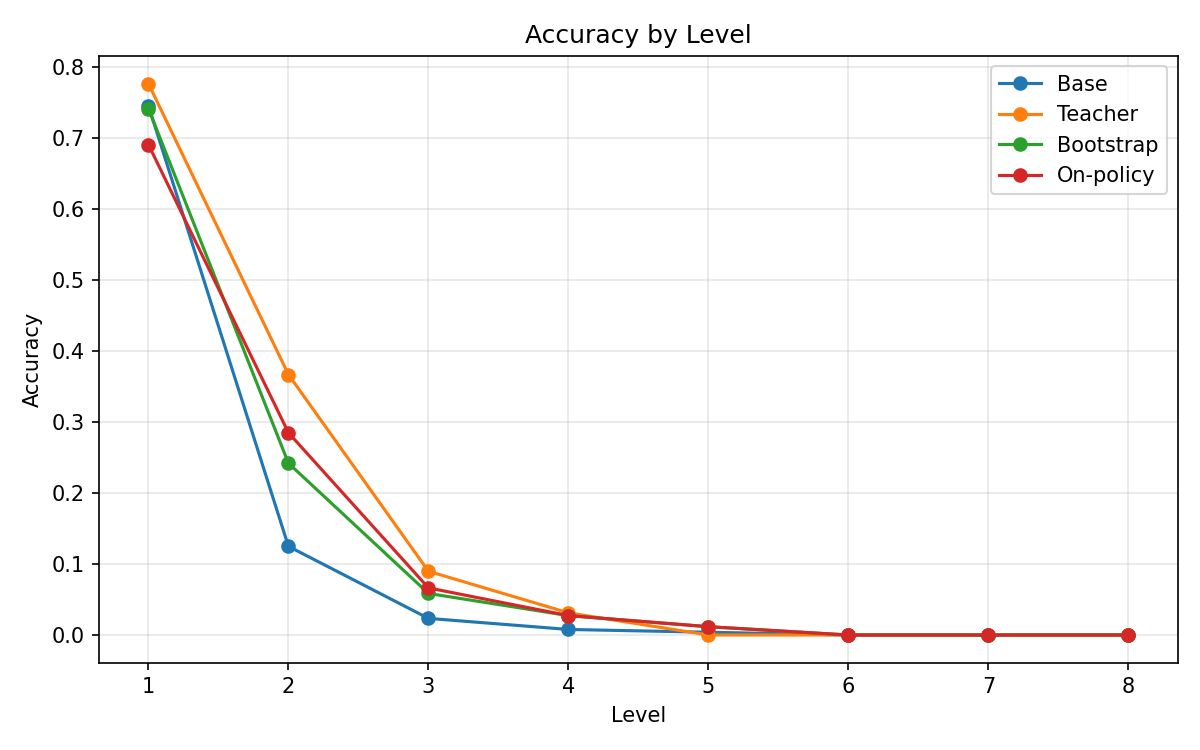
\includegraphics[width=0.8\textwidth]{imgs/data.png}
\caption{Accuracy comparing Off-policy and On-policy SFT methods}
\label{fig:data}
\end{figure}

Figure \ref{fig:data} shows the accuracy of different data sources.
Surprisingly, on-policy SFT performs worse than off-policy SFT with teacher generated data. This may suggest that the quality of data matter. The teacher model generates much more correct solutions compared to the base model.

We further support this hypothesis by applying different filtering strategies to the data to improve data quality.

\todo{insert table/figure of filtering strategies}


\section{Loss Function}
\begin{figure}[h!]
\centering
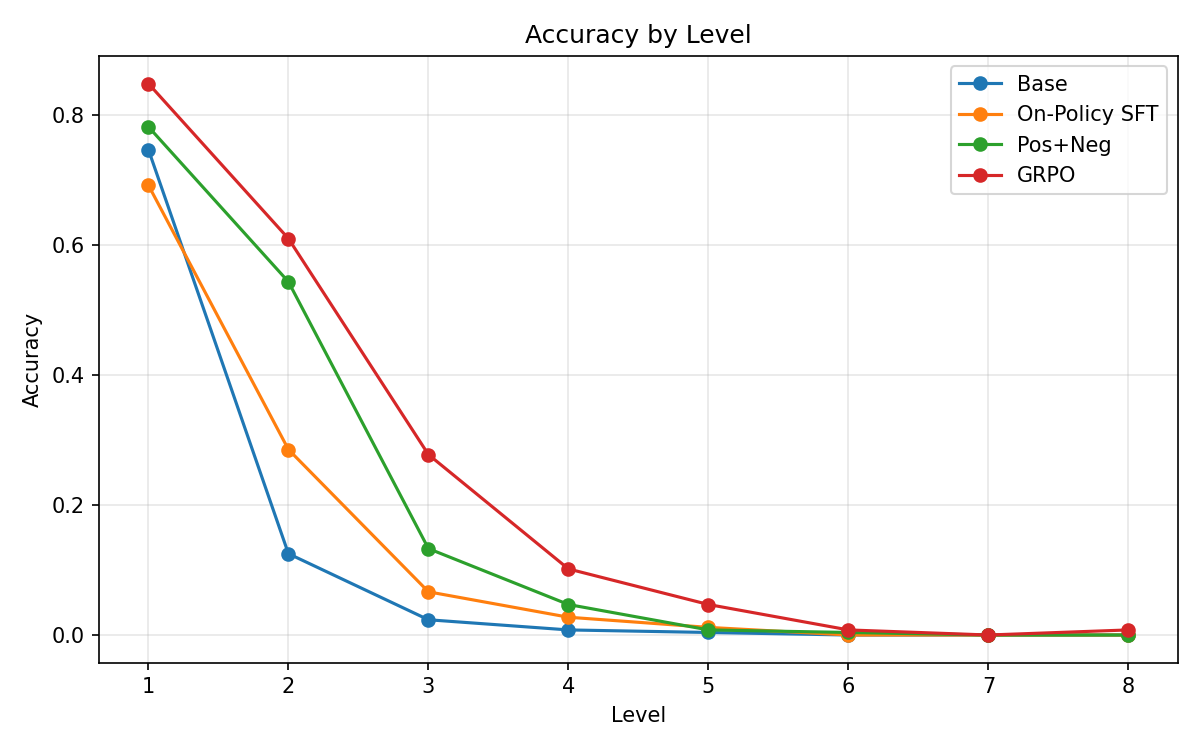
\includegraphics[width=0.8\textwidth]{imgs/loss_fn.png}
\caption{Accuracy comparing different loss functions under On-policy setting}
\label{fig:loss_fn}
\end{figure}

We find that after On-policy SFT training, the model's performance improves from the \textbf{Base} model. However, the gap between GRPO is still large. By adding negative samples, we see that we can recover the bulk of the performance gap. 

\todo{add results for REINFORCE with baseline}


\chapter{Transfer and Generality}
After isolating mechanisms on string composition, We perform two generalization checks:
\begin{itemize}
\item \textbf{Task transfer:} evaluate whether composition-trained models improve on broader math, code, and general reasoning benchmarks.
\item \textbf{Model-family transfer:} replicate key findings across model sizes and families (for example Llama and Qwen variants).
\end{itemize}

\todo{}


\chapter{Conclusion}
This thesis investigates compositional generalization as a mechanism-level post-training problem. In the controlled string-function setting, RL clearly outperforms off-policy SFT on deeper composition levels under matched compute. Attempts to improve off-policy SFT via filtering do not close this gap.

The evidence points to a structured explanation: on-policy data matters, negative samples likely matter, and some objective-level RL machinery may be optional depending on the regime. This motivates a decomposed view of RL rather than treating it as a monolithic method.

Practically, the work suggests a research path for designing cheaper and simpler training recipes that preserve compositional gains: start from on-policy supervised objectives, add explicit negative learning signals, and then layer in normalization or regularization only when needed.

More broadly, the thesis contributes a way to study reasoning emergence with controlled extrapolation metrics and component-wise interventions. The long-term goal is to convert empirical ``RL works'' observations into precise, transferable principles for building reasoning-capable language models.

%\appendix
%\include{appendix}

\backmatter

%\renewcommand{\baselinestretch}{1.0}\normalsize

% By default \bibsection is \chapter*, but we really want this to show
% up in the table of contents and pdf bookmarks.
\renewcommand{\bibsection}{\chapter{\bibname}}
%\renewcommand{\bibpreamble}{This text goes between the ``Bibliography''
%  header and the actual list of references}
\bibliographystyle{plainnat}
\bibliography{main} %your bib file

\end{document}
